\documentclass{article}

\usepackage{graphicx} %LaTeX package to import graphics
\usepackage{plantuml}

\graphicspath{{images/}} %configuring the graphicx package

\title{SafeCatChat \- Medical Professional Patient Communication}
\author{Alex Ramirez}
\date{April 4th, 2026}

\begin{document}
\maketitle

\tableofcontents

\section{Introduction}

The SafeCatChat application is intended to be a safe, secure, sovereign data platform
for medical professionals to communicate with their patients.  It is built with strict 
guidelines that can ensure the confidentiality, integrity, and availability of patient
data.

In this work package we will focus on creating the Medical Professional Patient Communication
View.  This view will provide a general overview of patient communication and statuses with
detailed information accessed by selecting or clicking on icons, links, etc.

\section{Functional Requirements}

The first set of functional requirements is illustrated in Figure 1.  
This wireframe was developed to provide a quick overview of a Medical Professional's 
Patients.  This view is the crucial entrypoint that all medical professionals will 
first see when they enter the application, and will use the most to manage their 
patient's health.\footnote{This is an educated guess and assumption at this time.  However, through the use of the Evidential platform plugin, we will test this hypothesis the ensure it is accurate and correct.}

This wireframe matches the following set of user stories:

\begin{quote}
    As a Medical Professional 
    I want to see at a glance my active patients for the day
    So that I know how many patients I will see
\end{quote}

\begin{figure}[h]
    \caption{Patients at a Glance View as a Medical Professional}\label{fig:messages-doctor-view}
    \centering
    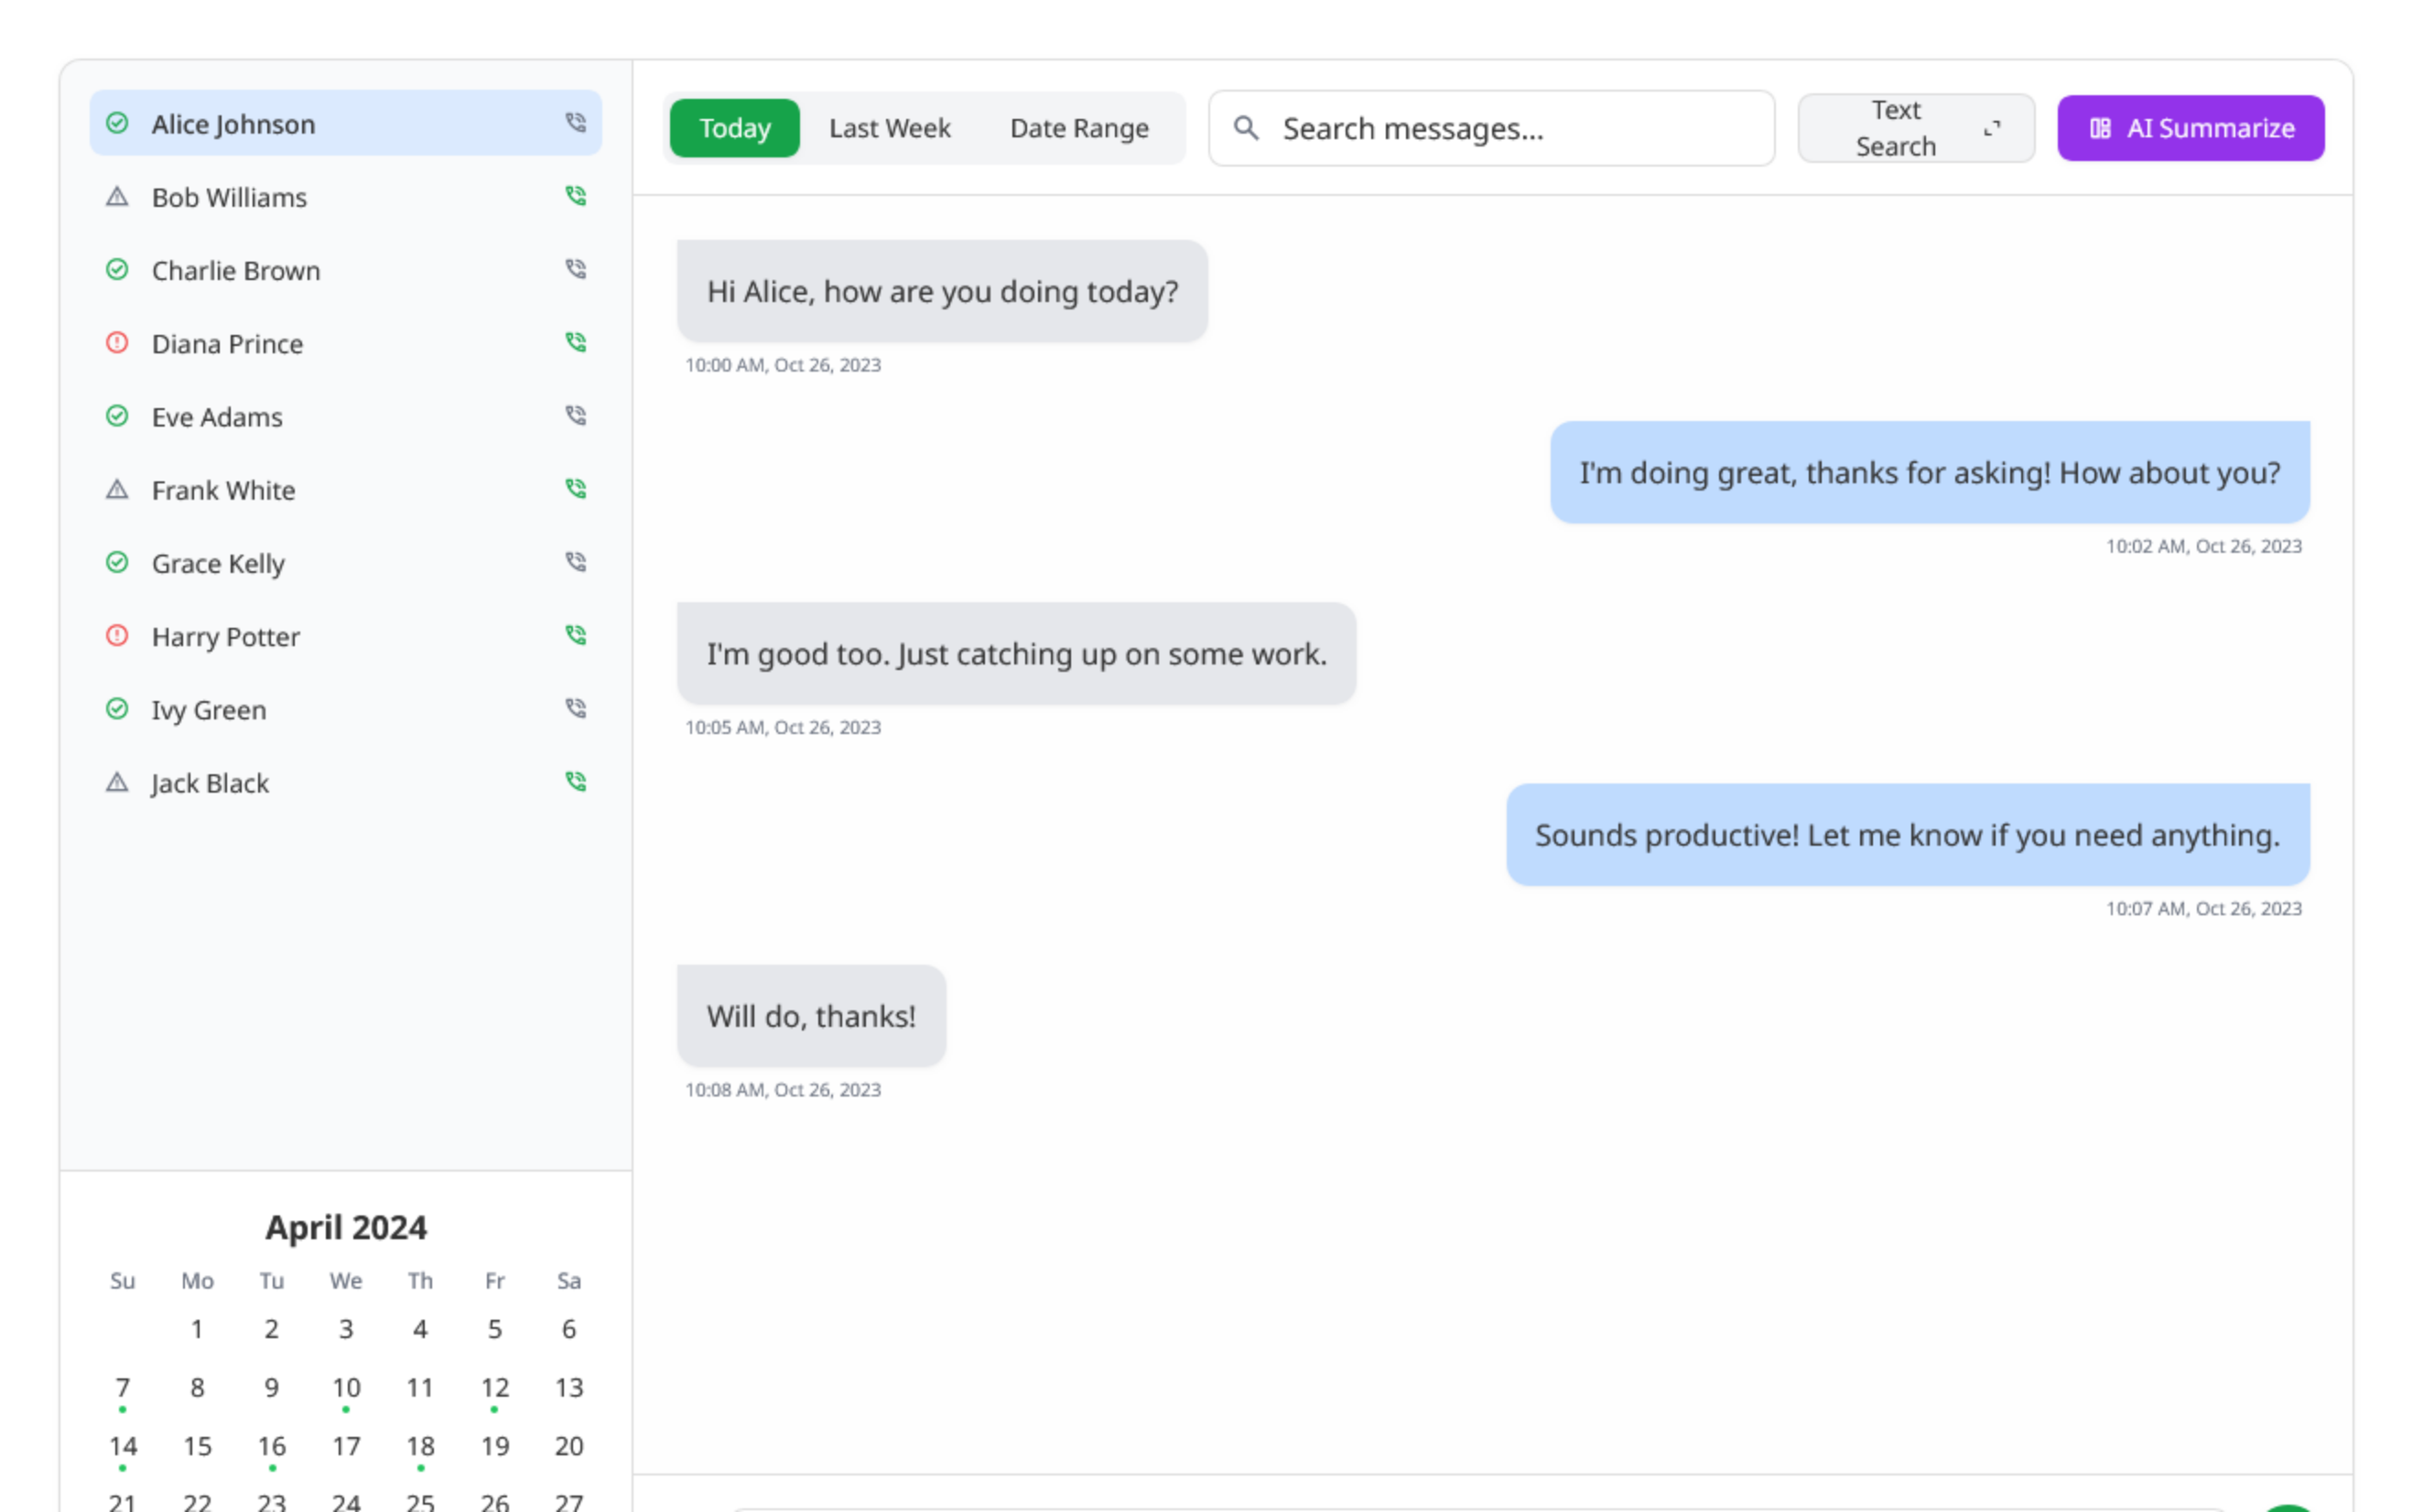
\includegraphics[width=1.0\textwidth]{messages-doctor-view}
\end{figure}

% 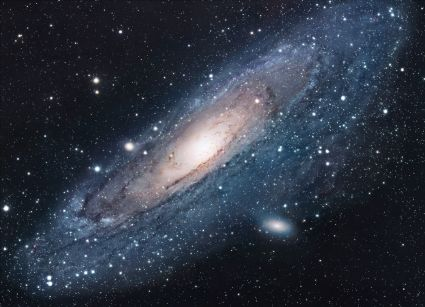
\includegraphics{universe} 
\subsection{Features}

% \begin{figure}[h]
%     \centering
%     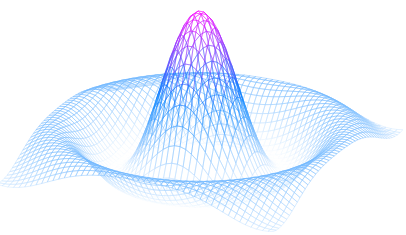
\includegraphics[width=0.75\textwidth]{mesh}
%     \caption{A nice plot.}\label{fig:mesh1}
% \end{figure}

\end{document}